\documentclass[addpoints,12pt]{exam}
%\documentclass[12pt]{article}
\usepackage[letterpaper, margin=0.75in]{geometry}
\usepackage{graphicx}
\usepackage{enumitem}
\usepackage{booktabs}
\usepackage{tabularx}

\begin{document}
\footer{}{Page \thepage\ of \numpages}{}

\begin{center}

\includegraphics[width=10cm]{../images/logo.png}
\end{center}

\begin{center}
\noindent{\LARGE Conceptual Physics \\ Homework Packet 6 \\Solutions \\}
\end{center}
 
\clearpage

\begin{flushright}
Score: \hspace{0.2in} / \numpoints ~ points
\end{flushright}

\begin{questions}
\question[6] Suppose you have a fair coin (\textit{i.e.} $P(\textrm{heads}) = 0.5$, $P(\textrm{tails}) = 0.5$).
\begin{parts}
\part What are the sixteen possible outcomes to tossing the coin four times? You can abbreviate, \textit{e.g.} HHTH as opposed to ``two heads followed by one tails followed by one heads.''
\begin{TheSolution}
\begin{tabular}{l l l l}
HHHH & HTHH & THHH & TTHH \\
HHHT & HTHT & THHT & TTHT \\
HHTH & HTTH & THTH & TTTH \\
HHTT & HTTT & THTT & TTTT \\
\end{tabular}
\end{TheSolution}
\part What is the probability of getting all tails?
\begin{TheSolution}
$1/2\times 1/2\times 1/2\times 1/2 = 1/16$
\end{TheSolution}
\part What is the probability of getting two heads and two tails in no particular order?
\begin{TheSolution}
There are 6 possible ways of getting two heads and two tails, out of 16 equally likely outcomes: P(two heads, two tails) = 6/16 = 3/8.
\end{TheSolution}
\end{parts}

\question[2] If a radioactive substance has a half-life of one year, does this mean that it will be completely decayed after two years? Explain.

From \textit{Light and Matter,} Chapter 33 Question 1.
\begin{TheSolution}
No, it means that after 2 years you would expect about $1/2 \times 1/2 = 1/4$ of the substance to remain.
\end{TheSolution}

\question[6] Suppose you have a sample of a radioactive substance that has a half-life of one year.
\begin{parts}
\part What fraction of the sample will have decayed after one year?
\begin{TheSolution}
One half.
\end{TheSolution}
\part What fraction of the sample will have decayed after two years?
\begin{TheSolution}
One half decays after one year; during the next year, one half of the remaining half decays, leaving one fourth of the radioactivity. This means three fourths of the sample will have decayed.
\end{TheSolution}
\part What fraction of the sample will have decayed after five years?
\begin{TheSolution}
$\frac{1}{2}\cdot\frac{1}{2}\cdot\frac{1}{2}\cdot\frac{1}{2}\cdot\frac{1}{2} = \frac{1}{32}$ of the radioactivity is left, meaning $\frac{31}{32}$ has decayed.
\end{TheSolution}
\end{parts}

\question[2] Three particles are traveling at the \textbf{same speed}. The waves of the three particles are as shown.
	\begin{center}
		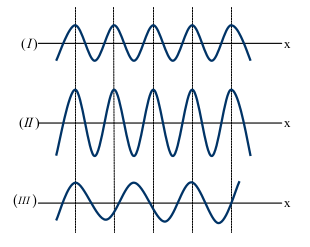
\includegraphics[width=3in]{../images/deBroglie.png}
	\end{center}
	Rank the \textbf{masses} of the particles ( I ), ( II ) and ( III ) by circling one of these six possibilities.
\begin{parts}
	\part $m_{II} > m_I > m_{III}$
	\part $m_{II} > m_{III} > m_I$
	\part $m_{I} = m_{II} > m_{III}$
	\part $m_{I} = m_{II} < m_{III}$
	\part $m_{II} > m_I = m_{III}$
	\part $m_{II} < m_I = m_{III}$
\end{parts}
\begin{TheSolution}
\textbf{C.} Since the velocities are all the same, the mass will impact the energy the particle has. The greater the energy, the smaller the wavelength: Therefore the greater the mass, the smaller the wavelength. Since (I) and (II) have the same wavelength (amplitude is irrelevant here) they must have the same mass. Since their wavelength is greater than (III), this means that they must have a greater mass than (III)
\end{TheSolution}

\question[4] A nuclear physicist is studying a nuclear reaction caused in
an accelerator experiment, with a beam of ions from the accelerator
striking a thin metal foil and causing nuclear reactions when a nucleus from one of the beam ions happens to hit one of the nuclei in
the target. After the experiment has been running for a few hours,
a few billion radioactive atoms have been produced, embedded in
the target. She does not know what nuclei are being produced, but
she suspects they are an isotope of some heavy element such as Pb,
Bi, Fr or U. Following one such experiment, she takes the target foil
out of the accelerator, sticks it in front of a detector, measures the
activity every 5 min, and makes a graph (bottom figure). Which element is it, given the following options? \textbf{Please explain your reasoning.}

From \textit{Light and Matter}, Chapter 33 Question 8


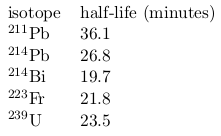
\includegraphics[height=1in]{../images/Isotopes.png}

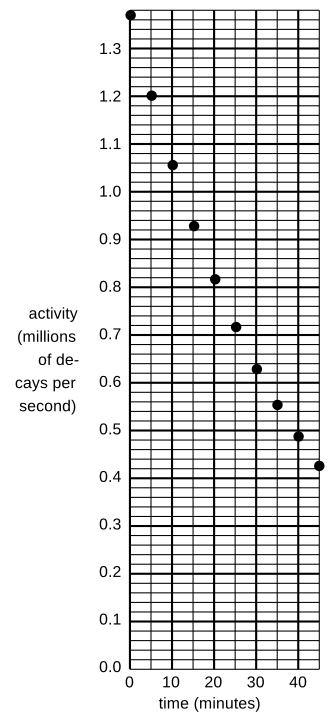
\includegraphics[height=6in]{../images/decay.png}
\begin{TheSolution}
Lead-214. The sample starts off with just under 1.4 million decays per second, so at its half-life it will have decayed to just under 0.7 million decays per second. This happens somewhere between 25 and 30 minutes, so $^{214}\texttt{Pb}$, which has a half-life of 26.8 minutes, is the most likely candidate.
\end{TheSolution}


\clearpage

%\question[4] When light is reflected from a mirror, perhaps only 80\% of the energy comes back. The rest is converted to heat. One could try to explain this in two different ways: (1) 80\% of the photons are reflected, or (2) all the photons are reflected, but each loses 20\% of its energy. Based on your everyday knowledge about mirrors, how can you tell which interpretation is correct?

%From \textit{Light and Matter}, Chapter 34 Question 3
\end{questions}



\end{document}